\RequirePackage[l2tabu, orthodox]{nag}
\documentclass[version=last, pagesize, twoside=off, bibliography=totoc, DIV=calc, fontsize=14pt, a4paper, french, english]{scrartcl}
%INSTALL
\pdfgentounicode=1 %permits (with package glyphtounicode) to copy eg x ⪰ y iff v(x) ≥ v(y) from pdf to unicode data. 
\input{glyphtounicode}%TODO avoid warning when redefining → (and others) ; make it work for ℝ (U+211D) as well
\usepackage[T1]{fontenc}%encode resulting accented characters correctly in resulting PDF, permits copy-paste
\usepackage[utf8]{inputenc}
\usepackage{newunicodechar}%able to use e.g. → or ≤ in source
\usepackage{lmodern}%has more characters such as ligatures, permit copy from resulting PDF.
\usepackage{textcomp}%useful for redefining → and ¬ and … (otherwise seems to attempt to use \textrightarrow and the like but are not defined)
% solves bug in lmodern, https://tex.stackexchange.com/a/261188/
\DeclareFontShape{OMX}{cmex}{m}{n}{
  <-7.5> cmex7
  <7.5-8.5> cmex8
  <8.5-9.5> cmex9
  <9.5-> cmex10
}{}

\SetSymbolFont{largesymbols}{normal}{OMX}{cmex}{m}{n}
\SetSymbolFont{largesymbols}{bold}  {OMX}{cmex}{m}{n}
%warn about missing characters
\tracinglostchars=2

%REDAC
\usepackage{booktabs}
\usepackage{calc}
\usepackage{tabularx}

\usepackage{etoolbox} %for addtocmd, newtoggle commands
\newtoggle{LCpres}
\togglefalse{LCpres}

\usepackage{mathtools} %load this before babel!
	\mathtoolsset{showonlyrefs,showmanualtags}

\usepackage{natbib}%Package frenchb asks to load natbib before babel/frenchb
\usepackage{babel}%[french, english]: language options should be on the document level
%suppresses the warning about frenchb not modifying the captions (“—” to “:” in “Figure 1 – Legend”).
%	\frenchbsetup{AutoSpacePunctuation=false,SuppressWarning=true}% test with false?
	\frenchbsetup{AutoSpacePunctuation=false,SuppressWarning=false}

%\usepackage[super]{nth}%better use fmtcount! (loaded by datetime anyway; see below about pbl with warnings and package silence)
\usepackage{listings} %typeset source code listings
	\lstset{language=XML,tabsize=2,captionpos=b,basicstyle=\NoAutoSpacing}%NoAutoSpacing avoids space before colon or ?}%,literate={"}{{\tt"}}1, keywordstyle=\fontspec{Latin Modern Mono Light}\textbf, emph={String, PreparedStatement}, emphstyle=\fontspec{Latin Modern Mono Light}\textbf, language=Java, basicstyle=\small\NoAutoSpacing\ttfamily, frame=single, aboveskip=0pt, belowskip=0pt, showstringspaces=false
\usepackage[nolist,smaller,printonlyused]{acronym}%,smaller option produces warnings from relsize in some cases, it seems.% Note silence and acronym and hyperref make (xe)latex crash when ac used in section (http://tex.stackexchange.com/questions/103483/strange-packages-interaction-acronyms-silence-hyperref), rather use \section{\texorpdfstring{\acs{UE}}{UE}}.
\usepackage{fmtcount}
\usepackage[nodayofweek]{datetime}%must be loaded after the babel package. However, loading it after {nth} generates a warning from fmtcount about ordinal being already defined. Better load it before nth? (then we can remove the silence package which creates possible crashes, see above.) Or remove nth?
%\usepackage{xspace}%do we need this?
\nottoggle{LCpres}{
	\usepackage[textsize=small]{todonotes}
}{
}
\iftoggle{LCpres}{
	%remove pdfusetitle (implied by beamer)
	\usepackage{hyperref}
}{
% option pdfusetitle must be introduced here, not in hypersetup.
	\usepackage[pdfusetitle]{hyperref}
}
\nottoggle{LCpres}{
%seems like authblk wants to be later than hyperref, but sooner than silence
\usepackage{authblk}
\renewcommand\Affilfont{\small}
}{
}
\usepackage{silence}
\WarningFilter{newunicodechar}{Redefining Unicode character}
%breaklinks makes links on multiple lines into different PDF links to the same target.
%colorlinks (false): Colors the text of links and anchors. The colors chosen depend on the the type of link. In spite of colored boxes, the colored text remains when printing.
%linkcolor=black: this leaves other links in colors, e.g. refs in green, don't print well.
%pdfborder (0 0 1, set to 0 0 0 if colorlinks): width of PDF link border
%hidelinks or: colorlinks, linkcolor=black, citecolor=black, urlcolor={blue!80!black}
\hypersetup{breaklinks, bookmarksopen}
%add hyperfigures=true in hypersetup (already defined in article mode)
\iftoggle{LCpres}{
	\hypersetup{hyperfigures}
}{
}

%in Beamer, sets url colored links but does not change the rest of the colors (http://tex.stackexchange.com/questions/13423/how-to-change-the-color-of-href-links-for-real)
%\hypersetup{breaklinks,bookmarksopen,colorlinks=true,urlcolor=blue,linkcolor=,hyperfigures=true}
% hyperref doc says: Package bookmark replaces hyperref’s bookmark organization by a new algorithm (...) Therefore I recommend using this package.
\usepackage{bookmark}

% center floats by default, but do not use with float
% \usepackage{floatrow}
% \makeatletter
% \g@addto@macro\@floatboxreset\centering
% \makeatother
\nottoggle{LCpres}{
	\usepackage{enumitem} %follow enumerate by a string saying how to display enumeration
}{
}
\usepackage{ragged2e} %new com­mands \Cen­ter­ing, \RaggedLeft, and \RaggedRight and new en­vi­ron­ments Cen­ter, FlushLeft, and FlushRight, which set ragged text and are eas­ily con­fig­urable to al­low hy­phen­ation (the cor­re­spond­ing com­mands in LaTeX, all of whose names are lower-case, pre­vent hy­phen­ation al­to­gether). 
\usepackage{siunitx} %[expproduct=tighttimes, decimalsymbol=comma] ou (plus récent ?) [round-mode=figures, round-precision=2, scientific-notation = engineering]
\sisetup{detect-all, locale = FR, strict}% to detect e.g. when in math mode (use a math font) - check whether this makes sense with strict
\usepackage{braket} %for \Set
\usepackage{doi}

\usepackage{amsmath,amsthm}
\usepackage{amssymb}% for \mathbb{R}
% \usepackage{amsfonts} %not required?
% \usepackage{dsfont} %for what?

\usepackage{environ}%for xdescwd command
%BUT see https://tex.stackexchange.com/questions/83798/cleveref-varioref-missing-endcsname-inserted for cleveref with french
\usepackage{cleveref}% cleveref should go "laster" than hyperref
%GRAPHICS
\usepackage{pgf}
\usepackage{pgfplots}
	\usetikzlibrary{babel, matrix, fit, plotmarks, calc, trees, shapes.geometric, positioning, plothandlers, arrows, shapes.multipart}
\pgfplotsset{compat=1.14}
\usepackage{graphicx}

\DeclareMathAlphabet\mathbfcal{OMS}{cmsy}{b}{n}

\graphicspath{{graphics/},{graphics-dm/}}
\DeclareGraphicsExtensions{.pdf}
\newcommand*{\IncludeGraphicsAux}[2]{%
	\XeTeXLinkBox{%
		\includegraphics#1{#2}%
	}%
}%

%HACKING
\usepackage{printlen}
\uselengthunit{mm}
% 	\newlength{\templ}% or LenTemp?
% 	\setlength{\templ}{6 pt}
% 	\printlength{\templ}
\usepackage{scrhack}% load at end. Corrects a bug in float package, which is outdated but might be used by other packages
\usepackage{mathrsfs}% for \mathscr

%Beamer-specific
%do not remove babel, which beamer uses (beamer uses the \translate command for the appendix); but french can be removed.
\iftoggle{LCpres}{
	\usepackage{appendixnumberbeamer}
	\setbeamertemplate{navigation symbols}{} 
	\usepackage{preamble/beamerthemeParisFrance}
	\usefonttheme{professionalfonts}
	\setcounter{tocdepth}{10}
	%From: http://tex.stackexchange.com/questions/168057/beamer-with-xelatex-on-texlive2013-enumerate-numbers-in-black
%I don’t think it’s useful to submit this as a bug: nothing has been solved since March, 2015. See: https://bitbucket.org/rivanvx/beamer/issues?status=resolved.

\setbeamertemplate{enumerate item}
{
  \begin{pgfpicture}{-1ex}{-0.65ex}{1ex}{1ex}
    \usebeamercolor[fg]{item projected}
    {\pgftransformscale{1.75}\pgftext{\normalsize\pgfuseshading{bigsphere}}}
    {\pgftransformshift{\pgfpoint{0pt}{0.5pt}}
      \pgftext{\usebeamercolor[fg]{item projected}\usebeamerfont*{item projected}\insertenumlabel}}
  \end{pgfpicture}%
}

\setbeamertemplate{enumerate subitem}
{
  \begin{pgfpicture}{-1ex}{-0.55ex}{1ex}{1ex}
    \usebeamercolor[fg]{subitem projected}
    {\pgftransformscale{1.4}\pgftext{\normalsize\pgfuseshading{bigsphere}}}
    \pgftext{%
      \usebeamercolor[fg]{subitem projected}%
      \usebeamerfont*{subitem projected}%
      \insertsubenumlabel}
  \end{pgfpicture}%
}

\setbeamertemplate{enumerate subsubitem}
{
  \begin{pgfpicture}{-1ex}{-0.55ex}{1ex}{1ex}
    \usebeamercolor[fg]{subsubitem projected}
    {\pgftransformscale{1.4}\pgftext{\normalsize\pgfuseshading{bigsphere}}}
    \pgftext{%
      \usebeamercolor[fg]{subsubitem projected}%
      \usebeamerfont*{subitem projected}%
      \insertsubsubenumlabel}
  \end{pgfpicture}%
}


}{
}
% \newcommand{\citep}{\cite}%Better: leave natbib.
% \setbeamersize{text margin left=0.1cm, text margin right=0.1cm} 
% \usetheme{BrusselsBelgium}%no, replace with paris
%\usetheme{ParisFrance}, no, usepackage better!
% Tex Gyre takes too much space, replace with Latin Modern Roman / Sans / Mono.
% Difference when loading explicitly Latin Modern Sans (compared to not using \setsansfont at all):
% the font LMSans17-Regular appears in the document;
% the title of the slides appears differently;
% it does not say (in the log file):
% > LaTeX Font Info:    Font shape `EU1/lmss/m/it' in size <10.95> not available
% > (Font)              Font shape `EU1/lmss/m/sl' tried instead on input line 85.
% > LaTeX Font Info:    Try loading font information for EU1+lmtt on input line 85.

%tikzposter-specific
%remove \usepackage{ragged2e}: causes 1=1 to be printed in the middle of the poster. (Anyway prints a warning about those characters being missing.)
%put [french, english] options next to \usepackage{babel} to avoid warning of 

\newcommand{\R}{ℝ}
\newcommand{\N}{ℕ}
\newcommand{\Z}{ℤ}
\newcommand{\card}[1]{\lvert{#1}\rvert}
\newcommand{\powerset}[1]{\mathscr{P}(#1)}%\mathscr rather than \mathcal: scr is rounder than cal (at least in XITS Math).
%powerset without zero
\newcommand{\powersetz}[1]{\mathscr{P}_\emptyset(#1)}
\newcommand{\suchthat}{\;\ifnum\currentgrouptype=16 \middle\fi|\;}
%\newcommand{\Rplus}{\reels^+\xspace}

\AtBeginDocument{%
	\renewcommand{\epsilon}{\varepsilon}
% we want straight form of \phi for mathematics, as recommended in UTR #25: Unicode support for mathematics.
%	\renewcommand{\phi}{\varphi}
}

% with amssymb, but I don’t want to use amssymb just for that.
% \newcommand{\restr}[2]{{#1}_{\restriction #2}}
%\newcommand{\restr}[2]{{#1\upharpoonright}_{#2}}
\newcommand{\restr}[2]{{#1|}_{#2}}%sometimes typed out incorrectly within \set.
%\newcommand{\restr}[2]{{#1}_{\vert #2}}%\vert errors when used within \Set and is typed out incorrectly within \set.
\DeclareMathOperator*{\argmax}{arg\,max}
\DeclareMathOperator*{\argmin}{arg\,min}


%Voting and MCDA
\newcommand{\allalts}{\mathscr{A}}
\newcommand{\alts}{A}
\newcommand{\allF}{\mathcal{F}}
\newcommand{\cat}[1]{C_{#1}}

%Voting
\newcommand{\feasalts}{F}
\newcommand{\allvoters}{\mathscr{N}}
\newcommand{\voters}{N}
\newcommand{\allsystems}{\mathcal{G}}
\newcommand{\preflarge}{\boldsymbol{\succeq}^\textbf{r}}%real, complete pref
\newcommand{\pref}{\boldsymbol{\succ}^\textbf{r}}%real, connected pref, strict
\newcommand{\ppreflarge}{\succeq^\text{p}}%partial pref
\newcommand{\ppref}{\succ^\text{p}}%partial pref
\newcommand{\prof}{(\boldsymbol{\succ}^\textbf{r}_i)_{i \in N}}
\newcommand{\profshort}{\boldsymbol{R}^\textbf{r}}
\newcommand{\profs}[1][]{\mathbfcal{R}^\textbf{r}\ifblank{#1}{}{_{#1}}}
\newcommand{\pprof}{(\succ_i^\text{p})_{i \in N}}
\newcommand{\pprofshort}{R^\text{p}}
\newcommand{\allprofs}{\mathcal{L}(\alts)^N}%\mathbfcal{R}
\newcommand{\anonprofs}{\mathcal{L}(\alts)^{N\setminus\set{i_0}}}%\mathbfcal{R}
\newcommand{\allpprofs}{\mathcal{O}(\alts)^N}
\newcommand{\linors}{\mathcal{L}(\alts)}
\newcommand{\pors}{\mathcal{O}(\alts)}%partial orders

\newcommand{\allsvs}{\intvl{0, m-1}^N}%all score-vectors
\usepackage{pdfrender}
\newcommand*{\boldgreek}[1]{%
  \textpdfrender{%
    TextRenderingMode=FillStroke,%
    LineWidth=.35pt,%
  }{#1}%
}
%Almost good: $x \text{\textpdfrender{TextRenderingMode=FillStroke,LineWidth=.35pt}{$\succcurlyeq$}\textsuperscript{\textbf{r}}} y$.
%Also: $x \textpdfrender{TextRenderingMode=FillStroke,LineWidth=.35pt}{\succcurlyeq} y$.

%\textpdfrender{TextRenderingMode=FillStroke,LineWidth=.35pt}{$\succcurlyeq$}\textsuperscript{\textbf{r}}
%\newcommand{\prefsv}{\textpdfrender{TextRenderingMode=FillStroke,LineWidth=.35pt}{\succcurlyeq}^\textbf{r}}%pref over score-vectors
\newcommand{\prefsv}{\mathrel{\text{\textpdfrender{TextRenderingMode=FillStroke,LineWidth=.15pt}{$\succcurlyeq$}\textsuperscript{\!\!\!s\textbf{\,r}}}}}%pref over score-vectors
\newcommand{\sprefsv}{\mathrel{\boldsymbol{\succ}^{\text{\!\!\!s}\textbf{\,r}}}}%strict pref over score-vectors
\newcommand{\iprefsv}{\mathrel{\boldsymbol{\sim}^{\text{\!\!\!s}\textbf{\,r}}}}%indiff, pref over score-vectors
\newcommand{\pprefsv}{\succcurlyeq^\text{\!\!\!s\,p}}%pref over score-vectors: our approximation
\newcommand{\psprefsv}{\succ^\text{\!\!\!s\,p}}%strict version
\newcommand{\piprefsv}{\sim^\text{\!\!\!s\,p}}

\newcommand{\probprofs}{P^\text{r}}
\newcommand{\probsvs}{P^\text{a}}

%logic atom
%⟼ (long)
\DeclareDocumentCommand{\lato}{ O{\prof} O{\alts} }{[#1 \!⟼\! #2]}
%logic atom in
%↝, \stackrel{\in}{\mapsto}, ➲, ⥹
\newcommand{\tightoverset}[2]{%
  \mathop{#2}\limits^{\vbox to -.5ex{\kern-0.9ex\hbox{$#1$}\vss}}}
\DeclareDocumentCommand{\latoin}{ O{\prof} O{\alpha} }{[#1 \tightoverset{\in}{⟼} #2]}
\newcommand{\alllang}{\mathcal{L}}
\newcommand{\ltru}{\texttt{T}}
\newcommand{\lfal}{\texttt{F}}
\newcommand{\laxiom}[1]{{\texgyreherosfamily{\textsc{#1}}}}

%ARG TH
\newcommand{\AF}{\mathcal{AF}}
\newcommand{\labelling}{\mathcal{L}}
\newcommand{\labin}{\textbf{in}\xspace}
\newcommand{\labout}{\textbf{out}}
\newcommand{\labund}{\textbf{undec}\xspace}
\newcommand{\nonemptyor}[2]{\ifthenelse{\equal{#1}{}}{#2}{#1}}
\newcommand{\gextlab}[2][]{
	\labelling{\mathcal{GE}}_{(#2, \nonemptyor{#1}{\ibeatsr{#2}})}
}
\newcommand{\allargs}{A^*}
\newcommand{\args}{A}
\newcommand{\ar}{a}
\newcommand{\ext}{\mathcal{E}}

%MCDA+Arg
\newcommand{\dm}{d}
\newcommand{\ileadsto}{\rightcurvedarrow}
\newcommand{\mleadsto}[1][\eta]{\rightcurvedarrow_{#1}}
\newcommand{\ibeats}{\vartriangleright}
\newcommand{\mbeats}[1][\eta]{\vartriangleright_{#1}}

%MISC
\newcommand{\lequiv}{\Vvdash}
\newcommand{\weightst}{W^{\,t}}

%MCDA classical
\newcommand{\crits}{\mathcal{J}}

%Sorting
\newcommand{\cats}{\mathcal{C}}
\newcommand{\catssubsets}{2^\cats}
\newcommand{\catgg}{\vartriangleright}
\newcommand{\catll}{\vartriangleleft}
\newcommand{\catleq}{\trianglelefteq}
\newcommand{\catgeq}{\trianglerighteq}
\newcommand{\alttoc}[2][x]{(#1 \xrightarrow{} #2)}
\newcommand{\alttocat}[3]{(#2 \xrightarrow{#1} #3)}
\newcommand{\alttoI}{(x \xrightarrow{} \left[\underline{C_x}, \overline{C_x}\right])}
\newcommand{\alttocatdm}[3][t]{\left(#2 \thinspace \raisebox{-3pt}{$\xrightarrow{#1}$}\thinspace #3\right)}
\newcommand{\alttocatatleast}[2]{\left(#1 \thinspace \raisebox{-3pt}{$\xrightarrow[]{≥}$}\thinspace #2\right)}
\newcommand{\alttocatatmost}[2]{\left(#1 \thinspace \raisebox{-3pt}{$\xrightarrow[]{≤}$}\thinspace #2\right)}

\definecolor{darkgreen}{rgb}{0,0.6,0}
\newcommand{\commentOC}[1]{{\small\color{blue}{\selectlanguage{french}$\big[$OC : #1$\big]$}}}
\newcommand{\commentSM}[1]{{\small\color{red}{\selectlanguage{french}$\big[$SM : #1$\big]$}}}
\newcommand{\commentPV}[1]{{\small\color{darkgreen}{\selectlanguage{french}$\big[$PV : #1$\big]$}}}
%\newcommand{\commentOC}[1]{{\selectlanguage{french}{\todo{OC : #1}}}}
%Or: \todo[color=green!40]
\newcommand{\innote}[1]{{\scriptsize{#1}}}

%this probably requires outdated float package, see doc KomaScript for an alternative.
% \newfloat{program}{t}{lop}
% \floatname{program}{PM}

%definition, theorem, lemma, example environments, qed trickery are only needed in article mode (not Beamer)
\nottoggle{LCpres}{
%style is plain by default (italic text)
	\newtheorem{definition}{Definition}
	\newtheorem{theorem}{Theorem}
%no italic: expected.
%http://tex.stackexchange.com/questions/144653/italicizing-of-amsthm-package
	\newtheorem{lemma}{Lemma}
%\crefname{axiom}{axiom}{axioms}%might be needed for workaround bug in cref when defining new theorems?

%\ifdefined\theorem\else
%\newtheorem{theorem}{\iflanguage{english}{Theorem}{Théorème}}
%\fi

\theoremstyle{remark}
	\newtheorem{examplex}{Example}
	\newtheorem{remarkx}{Remark}
	\newtheorem{factx}{Fact}

%trickery allowing use of \qedhere and the like.
\newenvironment{example}{
	\pushQED{\qed}\renewcommand{\qedsymbol}{$\triangle$}\examplex
}{
	\popQED\endexamplex
}
\newenvironment{fact}{
	\pushQED{\qed}\renewcommand{\qedsymbol}{$\triangle$}\factx
}{
	\popQED\endfactx
}
\newenvironment{remark}{
	\pushQED{\qed}\renewcommand{\qedsymbol}{$\triangle$}\remarkx
}{
	\popQED\endremarkx
}
}{
}
\crefname{examplex}{example}{examples}% I wonder why this is unnecessary in case of singular

%which line breaks are chosen: accept worse lines, therefore reducing risk of overfull lines. Default = 200
\tolerance=2000
%accept overfull hbox up to...
\hfuzz=2cm
%reduces verbosity about the bad line breaks
\hbadness 5000
%reduces verbosity about the underful vboxes
\vbadness=1300
%sloppy sets tolerance to 9999
\apptocmd{\sloppy}{\hbadness 10000\relax}{}{}

\bibliographystyle{abbrvnat}
%or \bibliographystyle{apalike} for presentations?

%doi package uses old-style dx.doi url, see 3.8 DOI system Proxy Server technical details, “Users may resolve DOI names that are structured to use the DOI system Proxy Server (http://doi.org (preferred) or http://dx.doi.org).”, https://www.doi.org/doi_handbook/3_Resolution.html
\makeatletter
\patchcmd{\@doi}{dx.doi.org}{doi.org}{}{}
\makeatother

% WRITING
%\newcommand{\ie}{i.e.\@\xspace}%to try
%\newcommand{\eg}{e.g.\@\xspace}
%\newcommand{\etal}{et al.\@\xspace}
\newcommand{\ie}{i.e.\ }
\newcommand{\eg}{e.g.\ }
\newcommand{\mkkOK}{\checkmark}%\color{green}{\checkmark}
\newcommand{\mkkREQ}{\ding{53}}%requires pifont?%\color{green}{\checkmark}
\newcommand{\mkkNO}{}%\text{\color{red}{\textsf{X}}}

\newlength{\xdescwd}
\makeatletter
\NewEnviron{xdesc}{%
  \setbox0=\vbox{\hbadness=\@M \global\xdescwd=0pt
    \def\item[##1]{%
      \settowidth\@tempdima{\textbf{##1}:}%
      \ifdim\@tempdima>\xdescwd \global\xdescwd=\@tempdima\fi}
  \BODY}
  \begin{description}[leftmargin=\dimexpr\xdescwd+.5em\relax,
    labelindent=0pt,labelsep=.5em,
    labelwidth=\xdescwd,align=left]\BODY\end{description}}
\makeatother

\makeatletter
\newcommand{\boldor}[2]{%
	\ifnum\strcmp{\f@series}{bx}=\z@
		#1%
	\else
		#2%
	\fi
}
\newcommand{\textstyleElProm}[1]{\boldor{\MakeUppercase{#1}}{\textsc{#1}}}
\makeatother
\newcommand{\electre}{\textstyleElProm{Électre}\xspace}
\newcommand{\electreIv}{\textstyleElProm{Électre Iv}\xspace}
\newcommand{\electreIV}{\textstyleElProm{Électre IV}\xspace}
\newcommand{\electreIII}{\textstyleElProm{Électre III}\xspace}
\newcommand{\electreTRI}{\textstyleElProm{Électre Tri}\xspace}
% \newcommand{\utadis}{\texorpdfstring{\textstyleElProm{utadis}\xspace}{UTADIS}}
% \newcommand{\utadisI}{\texorpdfstring{\textstyleElProm{utadis i}\xspace}{UTADIS I}}

%TODO
% \newcommand{\textstyleElProm}[1]{{\rmfamily\textsc{#1}}} 

\newunicodechar{ℝ}{\mathbb{R}}
\newunicodechar{≠}{\ensuremath{\neq}}
\newunicodechar{≤}{\ensuremath{\leq}}
\newunicodechar{≥}{\ensuremath{\geq}}
\newunicodechar{→}{\ifmmode\rightarrow\else\textrightarrow\fi}
\newunicodechar{⇒}{\ensuremath{\Rightarrow}}
\newunicodechar{⇔}{\ensuremath{\Leftrightarrow}}
\newunicodechar{∪}{\cup}
\newunicodechar{∩}{\cap}
\newunicodechar{∧}{\land}
\newunicodechar{∨}{\lor}
\newunicodechar{¬}{\ifmmode\lnot\else\textlnot\fi}
\newunicodechar{…}{\ifmmode\ldots\else\textellipsis\fi}
\newunicodechar{×}{\ifmmode\times\else\texttimes\fi}


%const
\newcommand{\tikzboxit}{\path node[draw, overlay, inner sep=0.6mm, fit=(boxed), rectangle] {};}%

\newlength{\GraphsNodeSep}
\setlength{\GraphsNodeSep}{7mm}

% MCDA Drawing Sorting
\newlength{\MCDSCatHeight}
\setlength{\MCDSCatHeight}{6mm}
\newlength{\MCDSAltHeight}
\setlength{\MCDSAltHeight}{4mm}
%separation between two vertical alts
\newlength{\MCDSAltSep}
\setlength{\MCDSAltSep}{2mm}
\newlength{\MCDSCatWidth}
\setlength{\MCDSCatWidth}{3cm}
\newlength{\MCDSAltWidth}
\setlength{\MCDSAltWidth}{2.5cm}
\newlength{\MCDSEvalRowHeight}
\setlength{\MCDSEvalRowHeight}{6mm}
\newlength{\MCDSAltsToCatsSep}
\setlength{\MCDSAltsToCatsSep}{1.5cm}
\newcounter{MCDSNbAlts}
\newcounter{MCDSNbCats}
\newlength{\MCDSArrowDownOffset}
\setlength{\MCDSArrowDownOffset}{0mm}

\tikzset{/Graphs/dot/.style={
	shape=circle, fill=black, inner sep=0, minimum size=1mm
}}
\tikzset{/MC/D/S/alt/.style={
	shape=rectangle, draw=black, inner sep=0, minimum height=\MCDSAltHeight, minimum width=\MCDSAltWidth
}}
\tikzset{MC/D/S/pref/.style={
	shape=ellipse, draw=gray, thick
}}
\tikzset{/MC/D/S/cat/.style={
	shape=rectangle, draw=black, inner sep=0, minimum height=\MCDSCatHeight, minimum width=\MCDSCatWidth
}}
\tikzset{/MC/D/S/evals matrix/.style={
	matrix, row sep=-\pgflinewidth, column sep=-\pgflinewidth, nodes={shape=rectangle, draw=black, inner sep=0mm, text depth=0.5ex, text height=1em, minimum height=\MCDSEvalRowHeight, minimum width=12mm}, nodes in empty cells, matrix of nodes, inner sep=0mm, outer sep=0mm, row 1/.style={nodes={draw=none, minimum height=0em, text height=, inner ysep=1mm}}
}}

\newlength{\GitCommitSep}
\setlength{\GitCommitSep}{13mm}

\tikzset{/Git/commit/.style={
	shape=rectangle, draw, minimum width=4em, minimum height=0.6cm
}}
\tikzset{/Git/branch/.style={
	shape=ellipse, draw, red
}}
\tikzset{/Git/head/.style={
	shape=ellipse, draw, fill=yellow
}}

\tikzset{profile matrix/.style={
	matrix of math nodes, column sep=3mm, row sep=2mm, nodes={inner sep=0.5mm, anchor=base}
}}
\tikzset{rank-profile matrix/.style={
	matrix of math nodes, column sep=3mm, row sep=2mm, nodes={anchor=base}, column 1/.style={nodes={inner sep=0.5mm}}, row 1/.style={nodes={inner sep=0.5mm}}
}}
\tikzset{rank-vector/.style={
	draw, rectangle, inner sep=0, outer sep=1mm
}}
\tikzset{isolated rank-vector/.style={
	draw, matrix of math nodes, column sep=3mm, inner sep=0, matrix anchor=base, nodes={anchor=base, inner sep=.33em}, ampersand replacement=\&
}}

% GUI
\tikzset{/GUI/button/.style={
	rectangle, very thick, rounded corners, draw=black, fill=black!40%, top color=black!70, bottom color=white
}}

% Logger objects
\tikzset{/logger/main/.style={
	shape=rectangle, draw=black, inner sep=1ex, minimum height=7mm
}}
\tikzset{/logger/helper/.style={
	shape=rectangle, draw=black, dashed, minimum height=7mm
}}
\tikzset{/logger/helper line/.style={
	<->, draw, dotted
}}

% Beliefs
\tikzset{/Beliefs/D/S/attacker/.style={
	shape=rectangle, draw, minimum size=8mm
}}
\tikzset{/Beliefs/D/S/supporter/.style={
	shape=circle, draw
}}

\newcommand{\tikzmark}[1]{%
	\tikz[overlay, remember picture, baseline=(#1.base)] \node (#1) {};%
}


\begin{acronym}
\acro{AMCD}{Aide Multicritère à la Décision}
\acro{ASA}{Argument Strength Assessment}
\acro{DA}{Decision Analysis}
\acro{DM}{Decision Maker}
\acro{DPr}{Deliberated Preferences}
\acro{DRSA}{Dominance-based Rough Set Approach}
\acro{DSS}{Decision Support Systems}
\acrodefplural{DSS}{Decision Support Systems}
% \newacroplural{DSS}[DSSes]{Decision Support Systems}
\acro{EJOR}{European Journal of Operational Research}
\acro{LNCS}{Lecture Notes in Computer Science}
\acro{MCDA}{Multicriteria Decision Aid}
\acro{MIP}{Mixed Integer Program}
\acro{NCSM}{Non Compensatory Sorting Model}
\acro{PL}{Programme Linéaire}
\acro{PLNE}{Programme Linéaire en Nombres Entiers}
\acro{PM}{Programme Mathématique}
\acro{MP}{Mathematical Program}
\acro{MIP}{Mixed Integer Program}
% \newacroplural{PM}{Programmes Mathématiques}
%acrodefplural since version 1.35, my debian has \ProvidesPackage{acronym}[2009/01/25, v1.34, Support for acronyms (Tobias Oetiker)]
\acrodefplural{PM}{Programmes Mathématiques}
\acro{PMML}{Predictive Model Markup Language}
\acro{RESS}{Reliability Engineering \& System Safety}
\acro{SMAA}{Stochastic Multicriteria Acceptability Analysis}
\acro{URPDM}{Uncertainty and Robustness in Planning and Decision Making}
\acro{XML}{Extensible Markup Language}
\end{acronym}


\begin{document}
\title{Simultaneous elicitation for voting rules}
\author{Olivier Cailloux}
\author{Stefano Moretti}
\affil{Université Paris-Dauphine, 
PSL Research University, 
CNRS, LAMSADE, 
75016 PARIS, FRANCE
}
\author{Paolo Viappiani\footnote{Authors are currently listed according to alphabetical order.}}
\affil{CNRS-LIP6 laboratory - Université Pierre-et-Marie-Curie (UPMC),
4, Place Jussieu 75252 Paris, France
}
\makeatletter
	\hypersetup{
		pdfsubject={Social choice},
		pdfkeywords={elicitation, active learning}
	}
\makeatother
\maketitle

\section{Introduction}
In some situations a committee may desire to select winning alternatives using the preferences, over those alternatives, of multiple individuals (called voters). For example, a jury may desire to use the opinions of multiple reviewers to elect the best papers among some given set of papers. We are interested in situations where the committee wants to express preferences on the voting rule and voters express preferences about the order of the alternatives. We assume the committee expresses only one voice: preference on the voting rule is consensual. Voters may have differing opinions however. The voting rule serves to aggregate those different opinions.

We assume the preferences on the voting rule (of the committee) and over alternatives (of the voters) are unknown and obtaining information about them have a cost. This could be because we care about privacy (knowing as few as necessary about other’s preferences might be considered good), because of transmission cost (?), because of cognitive cost or other resources required for someone to make up her preferences, including, in the case of the committee, the cost of coming to an agreement. Hence, we are interested in querying as few as possible.

We are interested in solving a given problem, meaning, finding (or getting close to) the set of winning alternatives, given a set of alternatives, a committee and a set of individuals with (well-defined but unknown) preferences. As a bonus however, we also obtain some reusable information about the voting rules the committee appreciates, which might be useful if the procedure has to be applied repeatedly with the same committee.

Here are some notations. In those notations, the relations in bold suffixed with the letter \textbf{r} indicate the “real” relations, which we want to distinguish from the approximations we will build (suffixed with the letter $p$ to indicate partial knowledge).
\begin{description}[font=\normalfont, leftmargin=!, labelwidth=\widthof{$F: \allprofs \rightarrow \powersetz{\alts}$}]
	\item[$N$] the (finite) set of voters
	\item[$\alts$] the (finite) set of alternatives, $\card{\alts} = m$
	\item[$\linors \subseteq \powerset{\alts × \alts}$] the linear orders (connected, transitive, asymmetric) on $\alts$
	\item[$\pors \subseteq \powerset{\alts × \alts}$] the partial orders (transitive, asymmetric) on $\alts$
	\item[$\pref_i \in \linors$] the preference of voter $i$ (called a complete preference)
	\item[$\ppref_i \in \pors$] a partial preference associated to $i$, representing our knowledge of $\pref_i$
	\item[$\prof = \profshort$] a profile of complete preferences, called a complete profile
	\item[$\pprof = \pprofshort$] a profile of partial preferences, called a partial profile
	\item[$\allprofs$] the set of all complete profiles
	\item[$\allpprofs$] the set of all partial profiles
	\item[$\powersetz{\alts}$] the set of all subsets of $\alts$ minus the emptyset
	\item[$F: \allprofs \rightarrow \powersetz{\alts}$] a voting rule (associates each complete profile to a non-empty subset of winning alternatives)
\end{description}

Throughout the article we consider defined a voting rule $G$ that is used to specify the preferences on the voting rule of the committee: given a complete profile $\prof$, the committee will select a winner among $G(\prof)$ (the tie-breaking being done in a way not described by $G$). We consider the committee is able to express some of its preferences under the form of constraints on $G$, such as: if $G$ selects such alternative given such profile, then it may not select such alternative given such profile.
When talking about some generic voting rule we use the letter $F$. 

We can extend the domain of a voting rule to all partial profiles instead of only complete profiles. Given a rule $F$, define the robust equivalent rule as $F^\text{robust}: \allpprofs → \powersetz{\alts}$ which selects all possible winners given the partial profile, thus, an alternative is in $F^\text{robust}(\pprof)$ if there exists a complete profile $\prof$ that is a completion of $\pprof$ (meaning that for each $i$, $\pref_i$ is a completion of $\ppref_i$) for which $F(\prof)$ selects that alternative.

\subsection{Voting rules select scoring-vectors}
Define a scoring-vector $x$ as an element of $\allsvs$, a mapping of voters to scores, where a score is an integer in $\intvl{0, m-1}$. (This notation designates intervals in the natural numbers throughout this article.) As $m$ is less than $10$ in our examples, we write our examples of scoring-vector as concatenated numbers, for example $43$ denotes a scoring-vector mapping the first voter to score $4$ and the second voter to score $3$.

Given a complete profile $\profshort = \prof$, we can associate each alternative $a$ to its scoring-vector $χ_{\profshort}(a) \in \allsvs$, by giving, for each voter $i \in N$, as many points to $a$ as the number of alternatives it is preferred to in $\pref_i$. Thus, $χ_{\profshort}$ is the function in $(\allsvs)^{A}$ that associates alternatives to scoring-vectors on the basis of the profile $\profshort$. 
We denote a scoring-vector as $x_a$ instead of $χ_{\profshort}(a)$ when the profile is clear from the context. 
For example, if $i$ puts $a$ last in her ranking $\pref_i$, $x_a$ maps $i$ to $0$. 
This is illustrated in \cref{fig:sv}.
\begin{figure}[t]
	\centering
	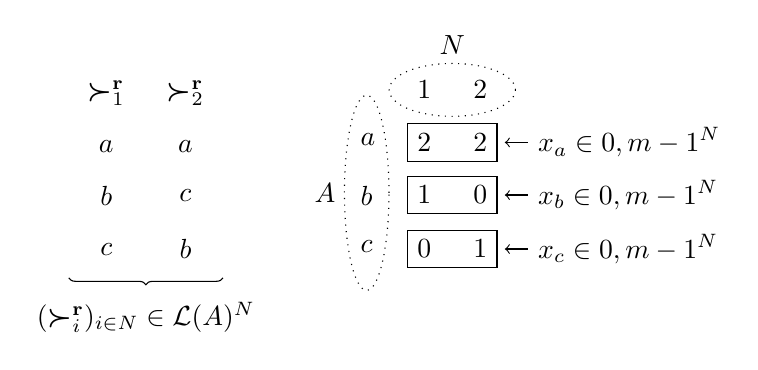
\begin{tikzpicture}
		\tikzset{prof matrix/.style={
			matrix, column sep=3mm, row sep=2mm
		}}
		\tikzset{rank-vector/.style={
			draw, rectangle, inner sep=0, outer sep=1mm
		}}
		
		\path node[prof matrix] (profile) {
			\path node {$\pref_1$};&
			\path node {$\pref_2$};
			\\
			\path node {$a$};&
			\path node {$a$};
			\\
			\path node {$b$};&
			\path node {$c$};
			\\
			\path node {$c$};&
			\path node {$b$};
			\\
		};
		\path[draw, decorate, decoration={brace, mirror}] (profile.south west) -- (profile.south east);
		\path ($(profile.south west)!.5!(profile.south east)$) ++ (0, -5mm) node {$\prof \in \linors^N$};
		
		\path (profile.north east) ++ (1.5cm, 0) node[prof matrix, anchor=north west] (rank-profile) {
			&
			\path node (header start) {1};&
			\path node (header end) {2};
			\\
			\path node (alts start) {$a$};&
			\path node (rv1 start) {2};&
			\path node (rv1 end) {2};
			\\
			\path node {$b$};&
			\path node (rv2 start) {1};&
			\path node (rv2 end) {0};
			\\
			\path node (alts end) {$c$};&
			\path node (rv3 start) {0};&
			\path node (rv3 end) {1};
			\\
		};
		\path node[draw, ellipse, dotted, inner sep=0, fit=(header start.north west) (header end.south east)] (N) {};
		\path (N.north) node[anchor=south, inner sep=1mm] {$N$};
		\path node[draw, ellipse, dotted, inner sep=0, fit=(alts start.north west) (alts end.south east)] (A) {};
		\path (A.west) node[anchor=east, inner sep=1mm] {$A$};
		\foreach \i/\a in {1/a, 2/b, 3/c} {
			\path node[rank-vector, fit=(rv\i\space start.north west) (rv\i\space end.south east)] (rv\i) {};
			\path[<-, draw] (rv\i.east) -- ++(0.3cm, 0) node[anchor=west] {$x_\a \in \allsvs$};
		}
	\end{tikzpicture}
	\caption{A complete profile and the corresponding scoring-vectors (adapted from \citet{cailloux_eliciting_2014})}
	\label{fig:sv}
\end{figure}

We say that a function in $(\allsvs)^{A}$ is a scoring-vectors profile iff it corresponds to some complete profile, thus, iff, for each voter, it gives different scores to different alternatives (viewing each column independently in \cref{fig:sv}, this forbids to repeat a number).
We can now view each complete profile as equivalent to its corresponding scoring-vectors profile: the just described mapping $\set{(\profshort, χ_{\profshort}), \profshort \in \allprofs}$ is a bijection.
We will thus use interchangeably $\profshort$ and $χ_{\profshort}$ when it causes no confusion, for example, we consider $F(χ_{\profshort})$ is defined (and equal to $F(\profshort)$).
We say that a complete profile $\profshort$ contains a scoring-vector iff some alternative is associated to this scoring-vector in $χ_{\profshort}$, that is, iff $x \in χ_{\profshort}(\allalts)$. 
We may also consider any voting rule $F$ interchangeably with its scoring-vectors voting rule counterpart $F^\text{s}$, that selects winning scoring-vectors given scoring-vectors profiles instead of winning alternatives given profiles. Indeed, given $F$, we can define $F^\text{s}(χ_{\profshort}) = χ_{\profshort}(F(\profshort))$, and this mapping is a bijection. Thus, we say that a scoring-vector $x$ wins in $F(\profshort)$, and write $x \in F(\profshort)$, to mean that $x \in F^\text{s}(χ_{\profshort})$. 

\section{Querying the preference on the voting rule through scoring-vectors}
We now want to define a way of querying whether, intuitively, $G$ (and thus, the committee) “considers” $x$ as a better scoring-vector than $y$. We will assume we can obtain information about this ordering (by interrogating the committee) and use this to enrich our knowledge of $G$.

Consider a binary relation $\prefsv$ over the scoring-vectors. Define $\sprefsv$ as its asymmetric part and $\iprefsv$ as its symmetric part. We ask queries of the form $x \prefsv y$, and we assume that the answers of the committee to those queries satisfy the following properties. First, when the committee tells us that $x \sprefsv y$, it implies that whenever both $x$ and $y$ are present in a profile, $y$ does not win in $G$. Second, when the committee tells us that $x \iprefsv y$, it implies that $x$ is selected by $G$ whenever $y$ is selected by $G$, for all profiles where both $x$ and $y$ are present. Third, $\prefsv$ is a preorder (a reflexive and transitive binary relation).

Let $\profs[xy] = \set{\profshort \suchthat \{x, y\} \subseteq χ_{\profshort}(\allalts)}$ denote the set of all complete profiles that contain the scoring-vectors $x$ and $y$. Given a rule $F$, $x \in \bigcup F(\profs[xy])$ holds whenever $F(\profshort)$ selects $x$ as one of the winners for some complete profile $\profshort$ that contains $x$ and $y$.

Our hypothesis is thus that $x \sprefsv y$ implies $y \notin \bigcup G(\profs[xy])$, that $\iprefsv$ implies $\forall \profshort \in \profs[xy]: x \in G(\profshort) ⇔ y \in G(\profshort)$, and that $\prefsv = \sprefsv ∪ \iprefsv$ is a preorder. (\Cref{sec:defSprefsv} analyzes alternative hypotheses.)

The transitivity of $\prefsv$ makes it a useful basis for queries: a few questions can bring “free” information, by computing the transitive closure of our knowledge so far.

Assume we are able to obtain $\psprefsv \subseteq \sprefsv$ and $\piprefsv \subseteq \iprefsv$, for some preorder $\pprefsv = \psprefsv ∪ \piprefsv$, $\psprefsv$ denoting the asymmetric part of $\pprefsv$. Define our approximation of $G$, $G_{\pprefsv}$, as the rule that selects the maximal elements according to $\pprefsv$, given a complete profile: $x$ wins in $G_{\pprefsv}(\profshort)$ iff there is no $y$ in $\profshort$ such that $y \psprefsv x$. The rule $G_{\pprefsv}$ gives us information about the real rule, $G$, in the sense that any real winner is in the winners selected by $G_{\pprefsv}$.
\begin{fact}
	Given $\pprefsv \subseteq \prefsv$, $\forall \profshort: G(\profshort) \subseteq G_{\pprefsv}(\profshort)$.
\end{fact}
\begin{proof}
	Consider $\profshort$ and assume $y$ does not win in $G_{\pprefsv}(\profshort)$. We show that $y$ does not win in $G(\profshort)$. We know that $y$ is dominated by some $x$ in $\profshort$, thus $x \psprefsv y$ and both $x$ and $y$ are in $\profshort$. Because $x \psprefsv y$, $x \sprefsv y$, thus $y$ does not win in $G(\profshort)$.
\end{proof}

A simpler way to obtain a preorder over $\allsvs$ useful for queries, adopted in a different article \citep{cailloux_eliciting_2014}, is to assume that the committee has such a relation “in mind”, and that this relation is a complete preorder. But this puts a restriction on $G$, as it has to be entirely compatible with such a way of thinking. Furthermore, it may be considered unclear what “having a relation in mind” mean in this context, if it is not precisely equated to conditions on $G$ as done here. The current approach also might be easier to include in more general elicitation procedures about voting rules.

\commentOC{On pourrait peut-être explorer la relation entre $G$ et $\prefsv$, voir la remarque ci-dessous.}

Remark that there are two properties in particular that we need, about $\prefsv$ and the relationship between $\prefsv$ and $G$: $\prefsv$ is a preorder, and $G \subseteq G_{\prefsv}$. Our definition of $\prefsv$, given $G$, permits to obtain the properties we want. However, we could relax our demands about $\prefsv$ and still obtain the desired properties. Consider as an example $m = 3$, one voter, and the pareto-compatible rule, which thus selects always the best ranked alternative, equivalently, which selects the scoring-vector $3$ as sole winner. Observe that $G$ determines according to our definitions a preorder where the scoring-vector $2$ is indifferent to $1$ (because both are dominated by $3$, and this is all that matters to $G$). Assume the committee tells us on the contrary that $2 \sprefsv 1$. We can still obtain the properties we want, although it contradicts our definition of $\sprefsv$.

\section{Characterisation of scoring-vector rules}
We define the class of rules that can be described as maximizing a preorder over scoring-vectors as preorder-based rules: a rule $F$ is a preorder-based rule iff for some preorder $\prefsv$ over $\allsvs$, $F = F_{\prefsv}$. A sub-class of this class is the class of weak-order based rules, corresponding to the case where $\prefsv$ is a weak-order.

\citet{cailloux_eliciting_2014} gave some preliminary analysis of those classes of rules.

\commentOC{Il pourrait être intéressant de poursuivre cette analyse. Et peut-être même utile pour une élicitation efficace ?}

\section{Elicitation of the preference on the voting rule only}
We assume we can observe $\sprefsv$ and $\iprefsv$: provided with a pair $x, y$, we can know whether $x \sprefsv y$, $y \sprefsv x$, $x \iprefsv y$, or none of those.

We start by assuming that $\prefsv$ is a weak-order (a complete preorder), thus “none of those” does not happen under this assumption.

We call a committee query a question in the form of a pair of scoring-vectors, to which we obtain as answer: $x \sprefsv y$, $y \sprefsv x$, or $x \iprefsv y$. We assume no noise in the answers: the answer we get conforms to the real relation $\prefsv$ as defined above.
We keep track of those answers by way of building iteratively a preorder $\pprefsv$.

We assume here that $\prof$ is not defined: we are interested in fully eliciting the preference on the voting rule of the committee, meaning, the function $G$, so that it can then be applied to any profile when they later arise. Note that we assume that the number of alternatives and voters are fixed (this follows from our definition of $G$).

We consider given a probability distribution $P^r$ over the complete profiles: $\sum_{\profshort \in \allprofs} \probprofs(\profshort) = 1$.

Define the badness $V_{\pprefsv}$ of our current approximation $\pprefsv$ as follows: $V_{\pprefsv} = \sum_{\profshort \in \allprofs} \probprofs(\profshort) \card{F_{\pprefsv}(\profshort)}$.

As further simplification hypotheses, we assume for now an impartial culture, thus all profiles are equally likely ($\probprofs$ is uniform); and we consider that the real rule $G$ is resolute, thus $\card{G(\profshort)}=1, \forall \profshort \in \allprofs$. These simplifications imply that $V_{\pprefsv} = \frac{1}{\card{\allprofs}} \card{F_{\pprefsv}(\profshort)}$ and that $V_{\pprefsv} = 1 ⇔ F_{\pprefsv} = G$.

Define $\probsvs_{\pprefsv}(x \sprefsv y)$ as our estimation, given our knowledge $\pprefsv$, of the probability that the committee answers $x \sprefsv y$ (this depends on some probability estimate over the set of possible weak-orders over scoring-vectors, probability estimate which in turn depends on $\pprefsv$, but which we do not need to make explicit for now). We define similarly $\probsvs_{\pprefsv}(x \iprefsv y)$.

We define the badness of asking a question of comparison of $x$ and $y$ as $b(x, y) = \probsvs_{\pprefsv}(x \sprefsv y) V_{\pprefsv ∪ \{(x, y)\}} + \probsvs_{\pprefsv}(y \sprefsv x) V_{\pprefsv ∪ \{(y, x)\}} + \probsvs_{\pprefsv}(x \iprefsv y) V_{\pprefsv ∪ \{(x, y), (y, x)\}}$. The lower, the better.

We need to find out how to compute $V_{\pprefsv}$, without having to iterate on the profiles: when $m=6, n=5$, $\card{\allprofs} = (6!)^5 > 10^{14}$.

Given two disjoint sets $B, C \subseteq \allsvs$ of scoring-vectors, define the number of profiles that contain all scoring-vectors from $B$ and no scoring-vectors from $C$ as $\#_{B, ¬C}$. Observe that $\#_B = \#_{B, ¬\emptyset} = [(m-\card{B})!]^n$, or $0$ if the scoring-vectors in $B$ are incompatible. Or, assuming all are compatible: $\binom{m^n - b}{m-b}$. Assuming they are compatible, the results depend only on the cardinals of $B$ and $C$, thus we can write it using these numbers. 
Observe that $\#_{3, ¬1} = \#_3 − \#_4$, $\#_{2, ¬2} = \#_2 − \#_4 − \#_{3, ¬1} − \#_{3, ¬1}$. 
We see that $\#{b, ¬c} = \#_b − (\sum_{1 ≤ k ≤ c} \binom{c}{k} \#_{b+k, ¬(c-k)})$.

Let’s decompose the preorder $\pprefsv$ into equivalence classes, one per “level”, where the level 1 contains the maximal scoring-vectors of $\pprefsv$, the level 2 contains the next best scoring-vectors, and so on. Write $z$ the last level of $\pprefsv$. Write $\alpha(l)$ the number of scoring-vectors at level $l$, $\beta(l)$ the number of scoring-vectors that are better than those at level $l$, thus $\beta(l) = \sum_{1 ≤ k < l} \alpha(k)$. Now $V_{\pprefsv} = \sum_{1 ≤ l ≤ z}\sum_{1 ≤ k ≤ \alpha(l)} k \#_{k, ¬(\alpha(l) - k + \beta(l))}$. Or, more likely, $V_{\pprefsv} = \sum_{1 ≤ l ≤ z}\sum_{1 ≤ k ≤ \alpha(l)} \binom{\alpha(l)}{k} k \#_{k, ¬(\alpha(l) - k + \beta(l))}$. \emph{Except} this does not account for the cases where some of these rank-vectors are incompatible.

\section{Simultaneous elicitation}
We call an individual query a question in the form of a pair of alternatives and a voter $i \in N$. We assume the answer is true, thus, conforms to the real relation $\pref_i$. We keep track of those answers by building iteratively a set of relations $\pprof$.

At each point in time we know $\pprefsv \subseteq \prefsv$ and $\ppref_i \subseteq \pref_i, \forall i \in N$, and hence, $F(\prof) \subseteq F_{\pprefsv}(\pprof)$.

We want to ask questions in a way that we get close to the real winners, $W = F(\prof)$, using few queries.

\bibliography{elic.bib}

\appendix
\section{About the definition of the relation over scoring-vectors}
\label{sec:defSprefsv}
Define binary relations over $\allsvs$ as follows.
\begin{itemize}
	\item $x B_> y$ iff $y \notin \bigcup G(\profs[xy]) ∧ x \in \bigcup G(\profs[xy])$
	\item $x B_\text{b} y$ iff $y \in \bigcup G(\profs[xy]) ∧ x \in \bigcup G(\profs[xy])$ (the letter b stands for “both”)
	\item $x B_\text{n} y$ iff $y \notin \bigcup G(\profs[xy]) ∧ x \notin \bigcup G(\profs[xy])$ (the letter n stands for “neither”)
	\item $x B_\text{w} y$ iff $x B_> y ∨ x B_\text{b} y$ iff $x \in \bigcup G(\profs[xy])$ (the letter w stands for “weak”)
	\item $x B^T y$, for any relation $B$, equals the transitive closure of $B$.
\end{itemize}

Note that we can’t suppose in general that $x \sprefsv y ⇔ y \notin \bigcup G(\profs[xy])$, as then $x \sprefsv y \sprefsv x$ for incompatible scoring-vectors. Also, we can’t suppose in general that $\sprefsv = B_>$. First, because $B_>$ may not be a strict partial order, and taking its transitive closure may not solve the problem: $G$ could be such that $(x = 21) B_> (y = 12) B_> (z = 20) B_> (w = 02) B_> (x = 12)$. The second inadequacy of $B_>$ is that sometimes, $x \sprefsv y$ seems intuitively meaningful even though $x$ and $y$ can’t be together in a profile: consider $44$ and $41$. In that case, a plausible interpretation of the intuition is that $44$ is better than a third scoring-vector, itself better than $41$ (and that no cycle happen): consider $44 B_> 33 B_> 41$.

We obtain the following possible definition relating the relation $\sprefsv$ and the rule $G$: $x \sprefsv y$ iff [($x B_> y$) or ($x B_>^T y$ and $x B_n y$)] and not $y B_\text{w}^T x$.

\end{document}

